\documentclass{article}
\usepackage[left=1in,right=1in,bottom=1in,top=1in]{geometry}
\usepackage[utf8]{inputenc}
\usepackage{amsmath}
\usepackage{amsfonts}
\usepackage{graphics}
\usepackage{tikz}
\usepackage{gensymb}
\usepackage{graphicx}
\usepackage{enumitem}
\usepackage{natbib}
 \usetikzlibrary{positioning}
\graphicspath{ {./}}
\title{MAP working paper}
\author{Tanvi Jindal, Yili Luo }
\date{}

\begin{document}

\maketitle

\section{Introduction}
Automobiles are arguably the most popular and important mode of transportation, with over 270 million vehicles registered in the United States alone.  Data from National Highway Traffic Safety Administration (NHTSA), the Centers for Disease Control and Prevention (CDC), and the Federal Motor Carrier Safety Administration (FMCSA) show that car crashes are the leading cause of death for young people between ages 15 and 29, and more than 30,000 Americans die each year in vehicle accidents \citep{Beltz2018}. To better understand vehicular collisions, scholars have developed numerous methods for measuring collision risk. Among the most popular are time-based methods, which are designed to capture how near or far a particular vehicle is from collision at any instant.  In this manuscript we focus on time-based measures, beggining with a review of previous work, then proposing a new metric for general two-dimensional scenarios, and concluding with an application of our metric to data from a driving simulator experiment assessing vehicle-to-vehicle alert characteristics. 

One of the most widely used methods of assessing collision risk is Time-To-Collision (TTC), which measures the ``time required for two vehicles to collide if they continue at their present speeds and on the same path" \citep{Hayward}. Since its inception, many extensions and refinements to TTC have been proposed.  Brown (2005) adjusted the measurement in one-dimensional scenarios using the velocity at collision to resolve the limitation of TTC being zero at collision regardless of severity.  \citet{Huo} developed algorithms for calculating TTC in two-dimensional freeway settings, using different geometric shapes to represent the driver's vehicle and a buffer area around the vehicle to match the driver's perception on collisions. \cite{Sobhani} studied right turning conflicts at intersections by grouping drivers by behavior and calculating TTC separately for each group. Nonetheless, these two-dimensional applications of TTC are limited to specific assumptions and scenarios, as a major limitation of TTC is that its values goes to infinity for non-collision trajectories.  Circumventing this limitation without imposing restrictive scenario-specific assumptions is difficult, and to our knowledge there has not been a TTC-like collision measure that can be applied uniformaly to two-dimensional settings.

An alternative to TTC, developed by \citet{Schwarz}, is Time of Closest Approach (TCA) measurement.  Instead of relying upon intersecting vehicle trajectories, TCA is based upon the distance between vehicles as a function of time, with TCA representing the time at which the minimum distance occurs. By using the distance between the vehicles, TCA avoids the propensity of TTC to yield infiinite values when vehicle trajectories are disjoint. However, TCA cannot be used to uniformly compare across different scenarios as the implications of ``minimum distance" are situation-dependent. Inspired by Brown's adjusted TTC, we decide to modify the calculation of TCA to produce a generalizable, time-based method of quantifying collisions in two-dimensions.  Our approach estimates vehicles trajectories and calculates the degree by which the trajectories would need to be shifted in order for the vehicles to collide, with smaller shifts indicating the original trajectory was closer to collision than larger shifts. This provides a robust measure that can be generally applied to two-dimensional scenarios to assess safety or collision severity.

To illustrate the usefulness of our metric, we apply it data from a driving simulator experiment collected by the National Advanced Driving Simulator (NADS), using simulator inputs to quantify collision proximity at a two-dimensional intersection crossing where drivers must react to avoid colliding with a vehicle running a red light.  In our application, we explore the effectiveness of using our measure to predict collision prior to impact, as well as potential advantages in statistical power that result from using our metric to retrospectively analyze experimental data.

\section{Methodology}

In this section we develop a metric for quantifying the proximity of two vehicles to collision. We begin with TCA as expressed by \citet{Schwarz}, and add complexity to better mirror real world scenarios. Then, we adjust the calculation of TCA by introducing vehicle-specific latent variables, which are used to measure proximity to collision.  Our development first considers vehicles as points, and later extends the method to consider vehicles as rectangles.

\subsection{Point collisions}

We first start by treating vehicles $P$ and $Q$ as point objects, introducing our notation using the diagram below:

\begin{center}
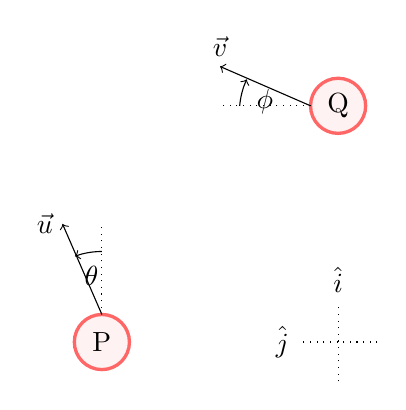
\begin{tikzpicture}
\centering
\filldraw[color=red!60, fill=red!5, very thick](-3,0) circle (0.35)node[anchor=center, black] {P};
\filldraw[color=red!60, fill=red!5, very thick](0,3) circle (0.35)node[anchor=center, black] {Q};
\draw[->] (-3, .35)-- (-3.5, 1.5)node[anchor=east] {$\vec{u}$};
\draw[dotted] (-3, .35)-- (-3, 1.5);
\draw[->] (-.35, 3)-- (-1.5, 3.5)node[anchor=south] {$\vec{v}$};
\draw[dotted] (-.35, 3)-- (-1.5, 3);
\draw [->](-3.00, 1.15) arc (90:110:1)node[anchor = north west, black] {$\theta$};
\draw [->](-1.25, 3.00) arc (175:155:1)node[anchor = north west, black] {$\phi$};
\draw [dotted] (.5, 0)--(-.5, 0)node[anchor=east] {$\hat{j}$};
\draw [dotted] (0, -.5)--(0, .5)node[anchor=south] {$\hat{i}$};
\end{tikzpicture}
\end{center}
Here, $\hat{i}$ and $\hat{j}$ are axes of the vector plane, and $\vec{u}$ and $\vec{v}$ are the velocities of P and Q respectively. $\theta$ is the angle of rotation of $\vec{u}$ at point P from $\hat{i}$, and $\phi$ is the angle of rotation of $\vec{v}$ at point Q from $\hat{j}$, as illustrated.  Notice, $\vec{u} = u_0 \cos(\theta)\hat{i} + u_0\sin(\theta)\hat{j}$, and $\vec{v}=-v_0\sin(\phi)\hat{i}+v_0\cos(\phi)\hat{j}$. 

For the purpose of this paper, we define anti-clockwise rotations to be positive and clockwise rotations to be negative. Therefore, with respect to illustration above, the angle $\theta$ is positive, and the angle $\phi$ is negative.

To calculate TCA for points $P$ and $Q$, we express the displacement from $P$ to $Q$ as a function of time. The value of time which minimizes this function is the TCA of $P$ and $Q$. Recognize that if $P$ and $Q$ collide with each other, their displacement at TCA will be 0.  We express $P$ and $Q$ at time $t$, using the following notation:
\begin{equation*}
    P(t) =
  \left( {\begin{array}{c}
   f_{\hat{i}}(t) \\
   f_{\hat{j}}(t) \\
  \end{array} } \right)
  \label{pt}
\end{equation*}
where $f_{\hat{i}}(t)= \int_0^t u_x(t)\cdot dt$ and $f_{\hat{j}}(t)= \int_0^t u_y(t)\cdot dt$ where $u_x(t)$ and $u_y(t)$ are the $\hat{i}$ and $\hat{j}$ components of point P's velocity, and
\begin{equation*}
    Q(t) =
  \left( {\begin{array}{c}
   g_x(t) \\
   g_y(t) \\
  \end{array} } \right)
  \label{qt}
\end{equation*}
where $g_x(t)= \int_0^t v_x(t)\cdot dt$ and $g_y(t)= \int_0^t v_y(t)\cdot dt$ where $v_x(t)$ and $v_y(t)$ are the $\hat{i}$ and $\hat{j}$ components of point Q's velocity. 

Thus the distance between $P$ and $Q$ at time $t$ can be expressed as $\vec{d}(t) = P(t) - Q(t)$, which can be used to define the time to closest approach, $TCA = \operatorname*{argmin}_t \{ \vec{d}(t) \}$.

\subsubsection{Simple model}

The simple model, as directly adopted from \citet{Schwarz}, assumes the positions of $P$ and $Q$ at time $t$ can be characterized by their initial positions $P_0$ and $Q_0$, and the constant velocity vectors $\vec{u}$ and $\vec{v}$:
\begin{equation}
    P(t) = P_0 + t\vec{u}
    \label{eqp}
\end{equation}
\begin{equation}
 Q(t) = Q_0 + t\vec{v}   
 \label{eqq}
\end{equation}
The distance, $\vec{d}(t)$, is then given by:
\begin{equation}
    \begin{split}
       \vec{d}(t) &= P(t) - Q(t) \\
       &= P_0 - Q_0 + (\vec{u} - \vec{v})t \\
       &= s + (\vec{u} - \vec{v})t
       \label{eqd}
    \end{split}
\end{equation}
where $s = P_0 - Q_0$.\\
TCA occurs when the magnitude of $\vec{d}(t)$ is minimum, requiring $d(t) = \sqrt{\vec{d}(t)\cdot\vec{d}(t)}$ to be minimized with respect to time.
\begin{equation}
   \frac{d}{dt}d(t) = \frac{(\vec{u} - \vec{v})\cdot(\vec{u} - \vec{v})t+2s(\vec{u} - \vec{v})}{\sqrt{(\vec{u} - \vec{v})\cdot(\vec{u} - \vec{v})t^2+2s(\vec{u} - \vec{v})t + s^2}}
    \notag
\end{equation}
Equating the derivative with provides a closed-form expression for the time to closest approach.
\begin{equation}
 TCA = \displaystyle \frac{- s_0}{|\vec{u} - \vec{v}|^2}
\end{equation}

\subsubsection{Acceleration and Turning}

The simple model enables a straightfoward calculation of TCA requiring relatively few inputs. However, this calculation is unable to reflect the important driver behaviors of braking, accelerating, and steering.

To modify the calculation to allow for variable velocity, we define the acceleration of $P$ as $\vec{a_P} = a_{P0}\cos(\theta)\hat{i} + a_{P0}\sin(\theta)\hat{j}$, and define the acceleration of $Q$ similarly.  Incorperating acceleration into component of velocity yields:
\begin{align*}
    \vec{u}(t) &= (u_0 + a_{P0}t) \cos(\theta){i} + (u_0 + a_{P0}t)\sin(\theta) \hat{j} \\
    \vec{v}(t) &= -(v_0+a_{Q0}t) \sin(\phi)\hat{i} + (v_0+a_{Q0}t)\cos(\phi)\hat{j}
\notag
\end{align*}

To further modify the calculation to allow for turning we use the steering wheel angle to determine change in vehicle heading using the steering ratio. Because turn of the wheel is the angle by which the vehicle turns at every instant, it can be viewed as the derivative of a vehicle's angle of motion.  Let turn of wheel of point P be $\omega_P$, then:
\begin{equation}
\omega_P = \frac{d\theta}{dt}   
 \label{eqwp}
\end{equation}
We assume $\omega_P$ is constant, so upon integrating both sides of equation (\ref{eqwp}) with respect to t, we get the angle of motion as a function of time as follows:\\
\begin{equation}
    \theta(t) = \omega_P \cdot t + \theta_0
    \notag
\end{equation}
where $\theta_0$ is the angle at which P was turned at time $t = 0$.\\
\begin{center}
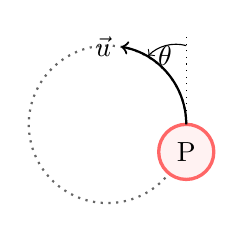
\begin{tikzpicture}
\filldraw[color=black!60, fill = white, dotted, thick] (-4, .35) circle (1);
\filldraw[color=red!60, fill=red!5, very thick](-3,0) circle (0.35)node[anchor=center, black] {P};
\draw[->, thick] (-3, .35) arc (0:80:1)node[anchor=east] {$\vec{u}$};
\draw[dotted] (-3, .35)-- (-3, 1.5);
\draw [->](-3.00, 1.35) arc (75:135:0.5)node[anchor = west, black] {$\theta$};
\end{tikzpicture}
\end{center}
As the illustration indicates, given a fixed steering wheel angle, point P travels with velocity $\vec{u}$ in a circular motion.  We point out that in most applications a complete revolution will not occur, and only the motion in the first quarter of the circle is relavent to the calculation.

\subsubsection{Standardized Degree of Collision Avoidance (SDCA)}

In the event that two vehicles do not collide, TCA indicates the time at which the distance between vehicles will be minimized based upon the set of driver inputs. However, it does not directly quantify the proximity of the two vehicles to a crash. Here, we define a \textit{reaction} as a fixed set of inputs.  We use this term because it might of particular interest to calculate TCA using vehicle trajectories upon having just realized the threat of collision.  The basis of our metric, Standardized Degree of Collision Avoidance (SDCA), is to measure how delayed a driver's reaction would need to be in order for the scenario to result in a collision. 

To approach this task, we begin by augmenting the expressions of $P(t)$ and $Q(t)$ by introducing two latent variables $Z_P$, which describes the reaction delay for $P$, and $Z_Q$, which describes the reaction delay for $Q$. This results in the adjusted positions functions $\tilde{P}(t)$ and $\tilde{P}(t)$:
\begin{equation}
    \tilde{P}(t) =
  \left( {\begin{array}{c}
   f_{\hat{i}}(t) + u_0\cdot\cos(\theta_0)\cdot Z_P\\
   f_{\hat{j}}(t) + u_0\cdot\sin(\theta_0)\cdot Z_P \\
  \end{array} } \right)
  \label{pdot}
\end{equation}

\begin{equation}
   \tilde{Q}(t) =
  \left( {\begin{array}{c}
   g_{\hat{i}}(t) - v_0\cdot\sin(\phi_0)\cdot Z_Q\\
   g_{\hat{j}}(t) + v_0\cdot\cos(\phi_0)\cdot Z_Q\\
  \end{array} } \right)
  \label{qdot}
\end{equation}

Equating, $\tilde{P}(t) = \tilde{Q}(t)$ for all t$\in\mathbb{R}$, and solving for $Z_P$ and $Z_Q$ yields the combinations of reaction delays by $P$ and $Q$ that would lead to a collision.  Thus, larger values of $Z_P$ and $Z_Q$ indicate a greater degree by which a collision was avoided.  We next seek to summarize the combinations of $Z_P$ and $Z_Q$ to provide a single overall measure of collision avoidance.

Setting $\tilde{P}(t) = \tilde{Q}(t)$ implies that $Z_P$ and $Z_Q$ can be expressed functions of time, with each value of $t$ corresponding to a pair $(Z_P(t), Z_Q(t) )$.  The pairs $(Z_P(t), Z_Q(t))$ can be viewed as a curve indexed by time, summarizing this curve amounts to summarizing all combinations of reaction delays that would have resulted in a collision. To summarize the curve, we calculate the expected distance, which we define as SDCA, from $(0,0)$ to the pairs $(Z_P(t), Z_Q(t))$. 

\begin{equation}
    \text{SDCA} = \frac{\int_{t_A}^{t_B} \sqrt{(Z_P(t) - 0)^2 + (Z_Q(t) - 0)^2} \cdot \sqrt{Z_P'(t)^2 + Z_Q'(t)^2} dt}{\int_{t_A}^{t_B} \sqrt{Z_P'(t)^2 + Z_Q'(t)^2} dt}
    \label{eqsdca}
\end{equation}

When performing this calculation, we restrict the curve to only include combinations occuring within the time indices defined by $t_A = \min(|Z_P|)$ and $t_B = \min(|Z_Q|)$.  In effect, this restriction excludes $(Z_P, Z_Q)$ combinations corresponding to large values of $t$ where our motion projections are unlikely to still resemble the actual trajectories of each vehicle.

\subsection{Object Collisions}

Treating vehicles as points has substantial mathematical and computational advantages, but it represents too much of a simplification for some applications that require greater precision.  In this section we outline the calculations of $TCA$ and $SDCA$ when vehicles are represented by rectangles. 

\subsubsection{TCA for Objects}

To begin, we use $P$ and $Q$ to denote the point at the center of each vehicle, we then define edges and corner points using each vehicles' length and width as defined in the diagram below:

\begin{center}
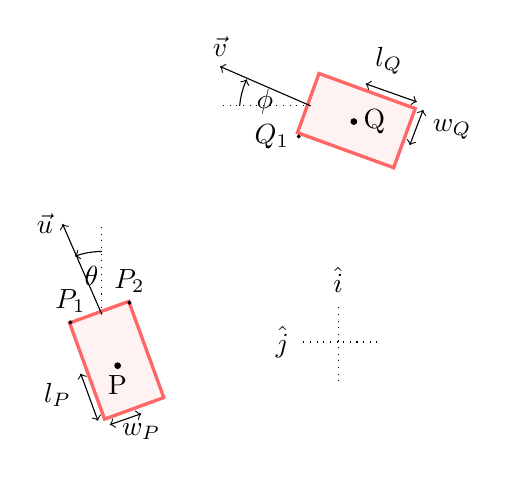
\begin{tikzpicture}
\filldraw[color=red!60, fill=red!5, very thick, rotate around={20:(-3, -0.3)}](-3.20,-0.95) rectangle (-2.40, 0.35)node[anchor= north west, black] {};
\filldraw[black] (-2.8, -0.30) circle (1pt) node[anchor=north] {P};
\filldraw[black] (-3.4, 0.25) circle (0.5pt) node[anchor=south] {$P_1$};
\filldraw[black] (-2.65, 0.5) circle (0.5pt) node[anchor=south] {$P_2$};
\draw[<->] (-3.05, -1)-- (-3.27, -0.4)node[anchor = north east]{$l_P$};
\draw[<->] (-2.9, -1.05)-- (-2.5, -0.91)node[anchor = north]{$w_P$};
\filldraw[color=red!60, fill=red!5, very thick, rotate around={-20:(0.3, 3)}](0.95, 3.20) rectangle (-0.35, 2.40) node[anchor=north, black] {};
\filldraw[black] (.20, 2.80) circle (1pt) node[anchor=west] {Q};
\filldraw[black] (-.5, 2.61) circle (0.5pt) node[anchor=east] {$Q_1$};
\draw[<->] (1, 3.05)-- (0.35, 3.28)node[anchor = south west]{$l_Q$};
\draw[<->] (.91, 2.5)-- (1.08, 2.95)node[anchor = north west]{$w_Q$};
\draw[->] (-3, .35)-- (-3.5, 1.5)node[anchor=east] {$\vec{u}$};
\draw[dotted] (-3, .35)-- (-3, 1.5);
\draw[->] (-.35, 3)-- (-1.5, 3.5)node[anchor=south] {$\vec{v}$};
\draw[dotted] (-.35, 3)-- (-1.5, 3);
\draw [->](-3.00, 1.15) arc (90:110:1)node[anchor = north west, black] {$\theta$};
\draw [->](-1.25, 3.00) arc (175:155:1)node[anchor = north west, black] {$\phi$};
\draw [dotted] (.5, 0)--(-.5, 0)node[anchor=east] {$\hat{j}$};
\draw [dotted] (0, -.5)--(0, .5)node[anchor=south] {$\hat{i}$};
\end{tikzpicture}
\end{center}
To calculate the time to closest approach (TCA) of vehicles $P$ and $Q$, we undertake the following steps: \\

\noindent1) Determine the corner points of the vehicle. For vehicle $P$, this is done by adding or subtracting the the $\vec{i}$ and $\vec{j}$ components of $l_P$ and $w_P$:
\begin{equation*}
P_k(t) = \begin{pmatrix}
f_{\hat{i}}(t) + (-1)^{k-k\bmod{3}} l_A\cos{\theta}+ (-1)^{\frac{k - k\bmod{2}}{2}+1} b_A \sin{\theta}\\
f_{\hat{j}}(t)+ (-1)^{k-k\bmod{3}} l_A\sin{\theta}+ (-1)^{\frac{k - k\bmod{2}}{2}} b_A \cos{\theta}
\end{pmatrix}
\end{equation*}

where k $\in \{1, 2, 3, 4\}$. Note, $\theta$ lies in the direction of $\hat{i}$, the formula for $Q_k$ is similar, but needs to be adjusted because $\phi$ lies in the direction of $\hat{j}$.\\

\noindent2) Find equations for all the edges of the vehicle. For any two corner points on an edge, we determine the vector equation of the line on which the edge lies. For example, the line joining $P_k$ and $P_{k+1}$ can be written as:
\begin{equation*}
A_k(t) = P_k(t) + (P_{k+1}(t)-P_k(t))\cdot\lambda_k
\end{equation*}

where $\lambda_k\in\mathbb{R}$ indicates position on $A_k$ relative to $P_k$, and $k + 1 = 1$ when $k = 4$. \\

\noindent3) Find the minimum distance from each corner point of one vehicle to each edge of the other vehicle. To find the minimum distance from a point $Q_{k*}$ to a line $A_k$, we first find the line passing through $Q_{k*}$ and perpendicular to $A_k$, which we label $N_k$. Then, we find, $m_k$, the point of intersection of $A_k$ and $N_k$ by equating $A_k$ and $N_k$. The minimum distance between line $A_k$, and corner point $Q_{k*}$ can be written as:\\
\[d_{k,k*}(t) =   \left\{
\begin{array}{ll}
      dist(Q_{k*}, m_k) & P_k\leq m_k\leq P_{k+1}\\
      \min\{dist(Q_{k*}, P_k), dist(Q_{k*}, P_{k+1})\} & otherwise \\
\end{array} 
\right. \]\\
where $dist(a, b)$ indicates distance between points a and b.\\ 

\noindent4) Minimize over all point-edge combinations of both vehicles to get TCA.  Each of the 32 point-line combinations has its own distance as a function of time. TCA is then found by finding the time at which the overall minimum distance, across all combinations, occurs. This could be done by taking $\mathcal{D}(t) = \min\{d_{1,1}, d_{1,2}, ..., d_{4,4}\}$, differentiating $\mathcal{D}(t)$, and solving for a minimum.  Or TCA could be approximated numerically using a grid search.

\subsubsection{SDCA for Objects}

When treating vehicles as points, SDCA was based upon adjusted driver reactions, which were characterized by introducing latent variables $Z_P$ and $Z_Q$ which provided modified positions $\tilde{P}(t)$ and $\tilde{Q}(t)$.  Because the rectangular representations of $P$ and $Q$ arise from center points, the calculation of SDCA in this framework can be approached similarly.  We outline the calculation below:

\noindent1) Modify the center points $P(t)$ and $Q(t)$ by introducing latent variables $Z_P$ and $Z_Q$, resulting in adjusted center points $\tilde{P}(t)$ and $\tilde{Q}(t)$. \\

\noindent2) Using the procedure described in Section 2.2.1, determine the adjusted corner points $\tilde{P}_k(t)$ and $\tilde{Q}_k(t)$, and use them to find distance functions $\{d_{1,1}, d_{1,2}, ..., d_{4,4}\}$ for each point-edge combination. \\

\noindent3) For each value of $t$, find the $(Z_P, Z_Q)$ pair closest to $(0,0)$ that results in at least one of the distances $\{d_{1,1}, d_{1,2}, ..., d_{4,4}\}$ equaling zero. This represents the minimum combined reaction delay that would result in vehicle $P$ colliding with vehicle $Q$. \\

\noindent4) Having obtained a curve of $(Z_P, Z_Q)$ pairs as a function of time in Step 3, we proceed to calculate $SDCA$ using Equation~\eqref{eqsdca}.

\section{Application}

To demonstrate the utility of $SCDA$, we apply the measure to driving simulator data collected by the NADS. In doing so, we illustrate two possible uses of $SDCA$. First, we see how SDCA can be used to forcast the occurrence of a collision based upon a vehicle's reaction profile. Second, we retrospectively analyze experimental data, replacing the binary outcome of collision/no collision using a numeric measure capable of capturing varying degrees of collision severity/avoidance.

\subsection{Data Description}

Haptic alerts are vibrations aimed drawing attention to a potentially dangerous situation. In this experiment, participants drove a simulated route while sitting on a custom haptic seat that could be controlled by the experimenters. The seat contained a 4x4 array of tactors used to convey alerts. Three different alert characteristics were manipulated, inter-pulse interval (IPI), intensity (INT), and directional pattern (DIP).  A randomized block design was used to allocate 180 participants into various experimental conditions, using IPI $= 0$, INT $= 50$ Hz, abd DIP $=$ "left only" as the default  condtions.  Within each block, one condition was varied, leaving the other two at their default values.  Additionally, the design included a control group, which did not receive an alert.

During the experiment, particpants drove on urban street with a posted speed limit of 35 mph, crossing three traffic signal-controlled intersections.  As they approached the third intersection, an incursion vehicle approached the intersection as cross-traffic from the left.  The incursion vehicle was created such that a collision was eminent if the participant did not react.  Roughly 4 seconds prior to collision the driver experienced a haptic alert, at which time the incursion vehicle was not yet visible.  Roughly 2.9 seconds prior to collision the vehicle became visible. 

Of these 180 participants who were randomized, 156 yielded time-series data suitable for analysis.  These data contain vehicle speed and heading angle collected at a rate of 60 frames per second. Additionally, a dummy variable recorded whether or not the participant collided with the incursion vehicle.

\subsection{SDCA Calculation}

In our analysis we use the time-series measurements of vehicle speed and heading angle to derive the scalar acceleration and turn of wheel variables needed to calculate $SDCA$ by determining the rates of change in speed and heading angle at every instance of time. We define $t_0$, the reaction start-point, to be the first time after the onset of the alert where the scalar acceleration or turn of wheel changes significantly. We defined a "significant change" as a rate of change larger than 0.3$^c$ for turn of wheel and larger than 3 m/s$^2$ for scalar acceleration. Based on the driving behaviors described by \cite{Hyden}, we split participants' reactions into five categories:\\
1. Scalar acceleration\\
2. Scalar deceleration\\
3. Turning\\
4. Scalar deceleration and turning\\
5. No reaction\\ 

Category 4, which is combination of two reactions, requires both acceleration and turn of wheel to significantly change within 0.167 seconds of each other. In this category the reaction start-point is determined by the first variable to significantly change.

Depending on which category the initial reaction falls under, we must determine the values of scalar acceleration or turn of wheel (or both) to use in the $SDCA$ calculation.  We do this using the average from the start of the reaction to the variable's maximum or minimum value.

\begin{figure}[h!]
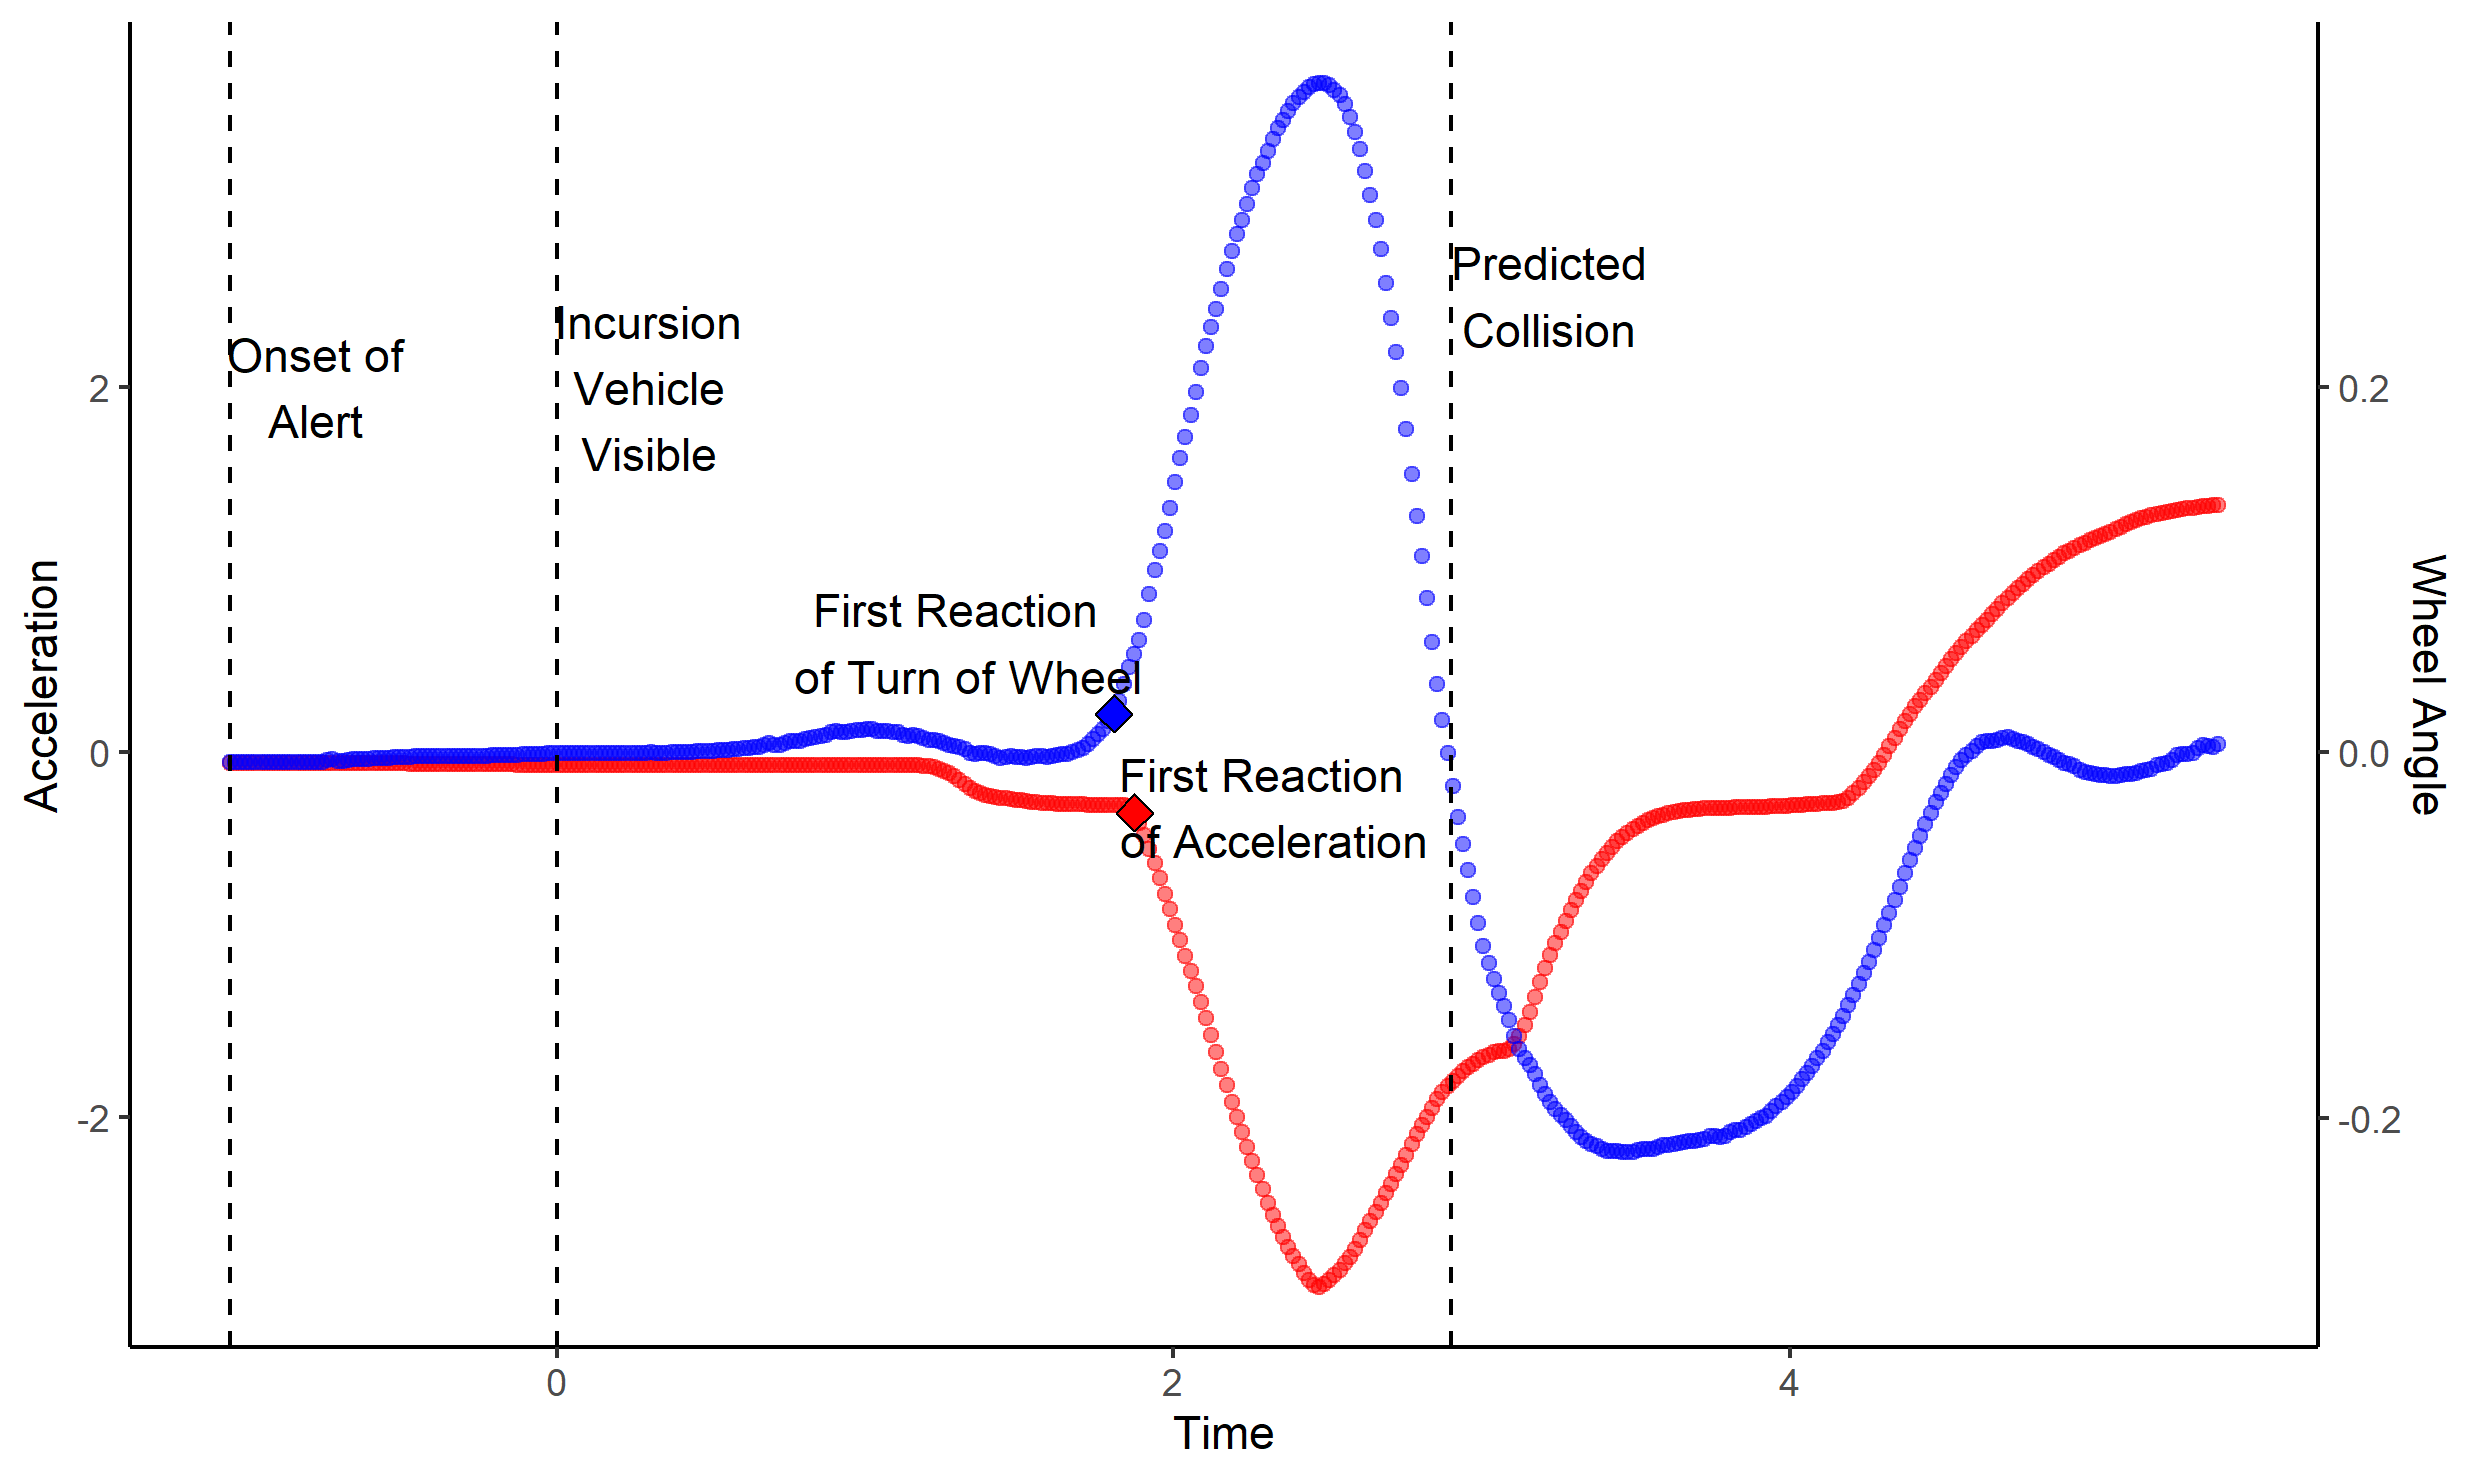
\includegraphics[width=\textwidth]{fig1.png}
\caption{Time Series Data for Participant 65}
\label{figure 1}
\end{figure}

Figure~\ref{figure 1} displays the time-series data for participant 65, with the scalar acceleration and turn of wheel shown in red and blue respectively for every time frame. For this participant, the start of their reaction is the time at which turn of wheel first changes significantly and marked accordingly on the graph. Because scalar acceleration changes significantly within 0.167 seconds, participant 65's reaction is classified into Category 4. Upon receiving this classification, we calculate the necessary inputs of acceleration and turn of wheel by taking their average values from the start of reaction to their minimum and maximum values respectively. 

We point out that this procedure creates a lag in when $SDCA$ can be calculated; however, $SDCA$ is still calculated prior to collision, and the amount of lag time could be reduced (potentially to zero) by determining reaction inputs differently.

Using the reaction start-points and the inputs described above are able to estimate the motion of each participant's vehicle. The incursion vehicle's motion is fixed, and easily accounted for. Using these charactizations, we calculate $SDCA$ for each participant via Equation~\eqref{eqsdca}. Because this calculation depends upon estimated quantities we denote the resultant value as $\hat{D}$, owing to the fact that it can vary depending upon how the reaction is estimated.  

\subsection{Forcasting Collision}

In this section we consider the use of $SDCA$ as a classifer, comparing $\hat{D}$ values of each participant with whether they collided with the incursion vehicle.

\begin{figure}[h!]
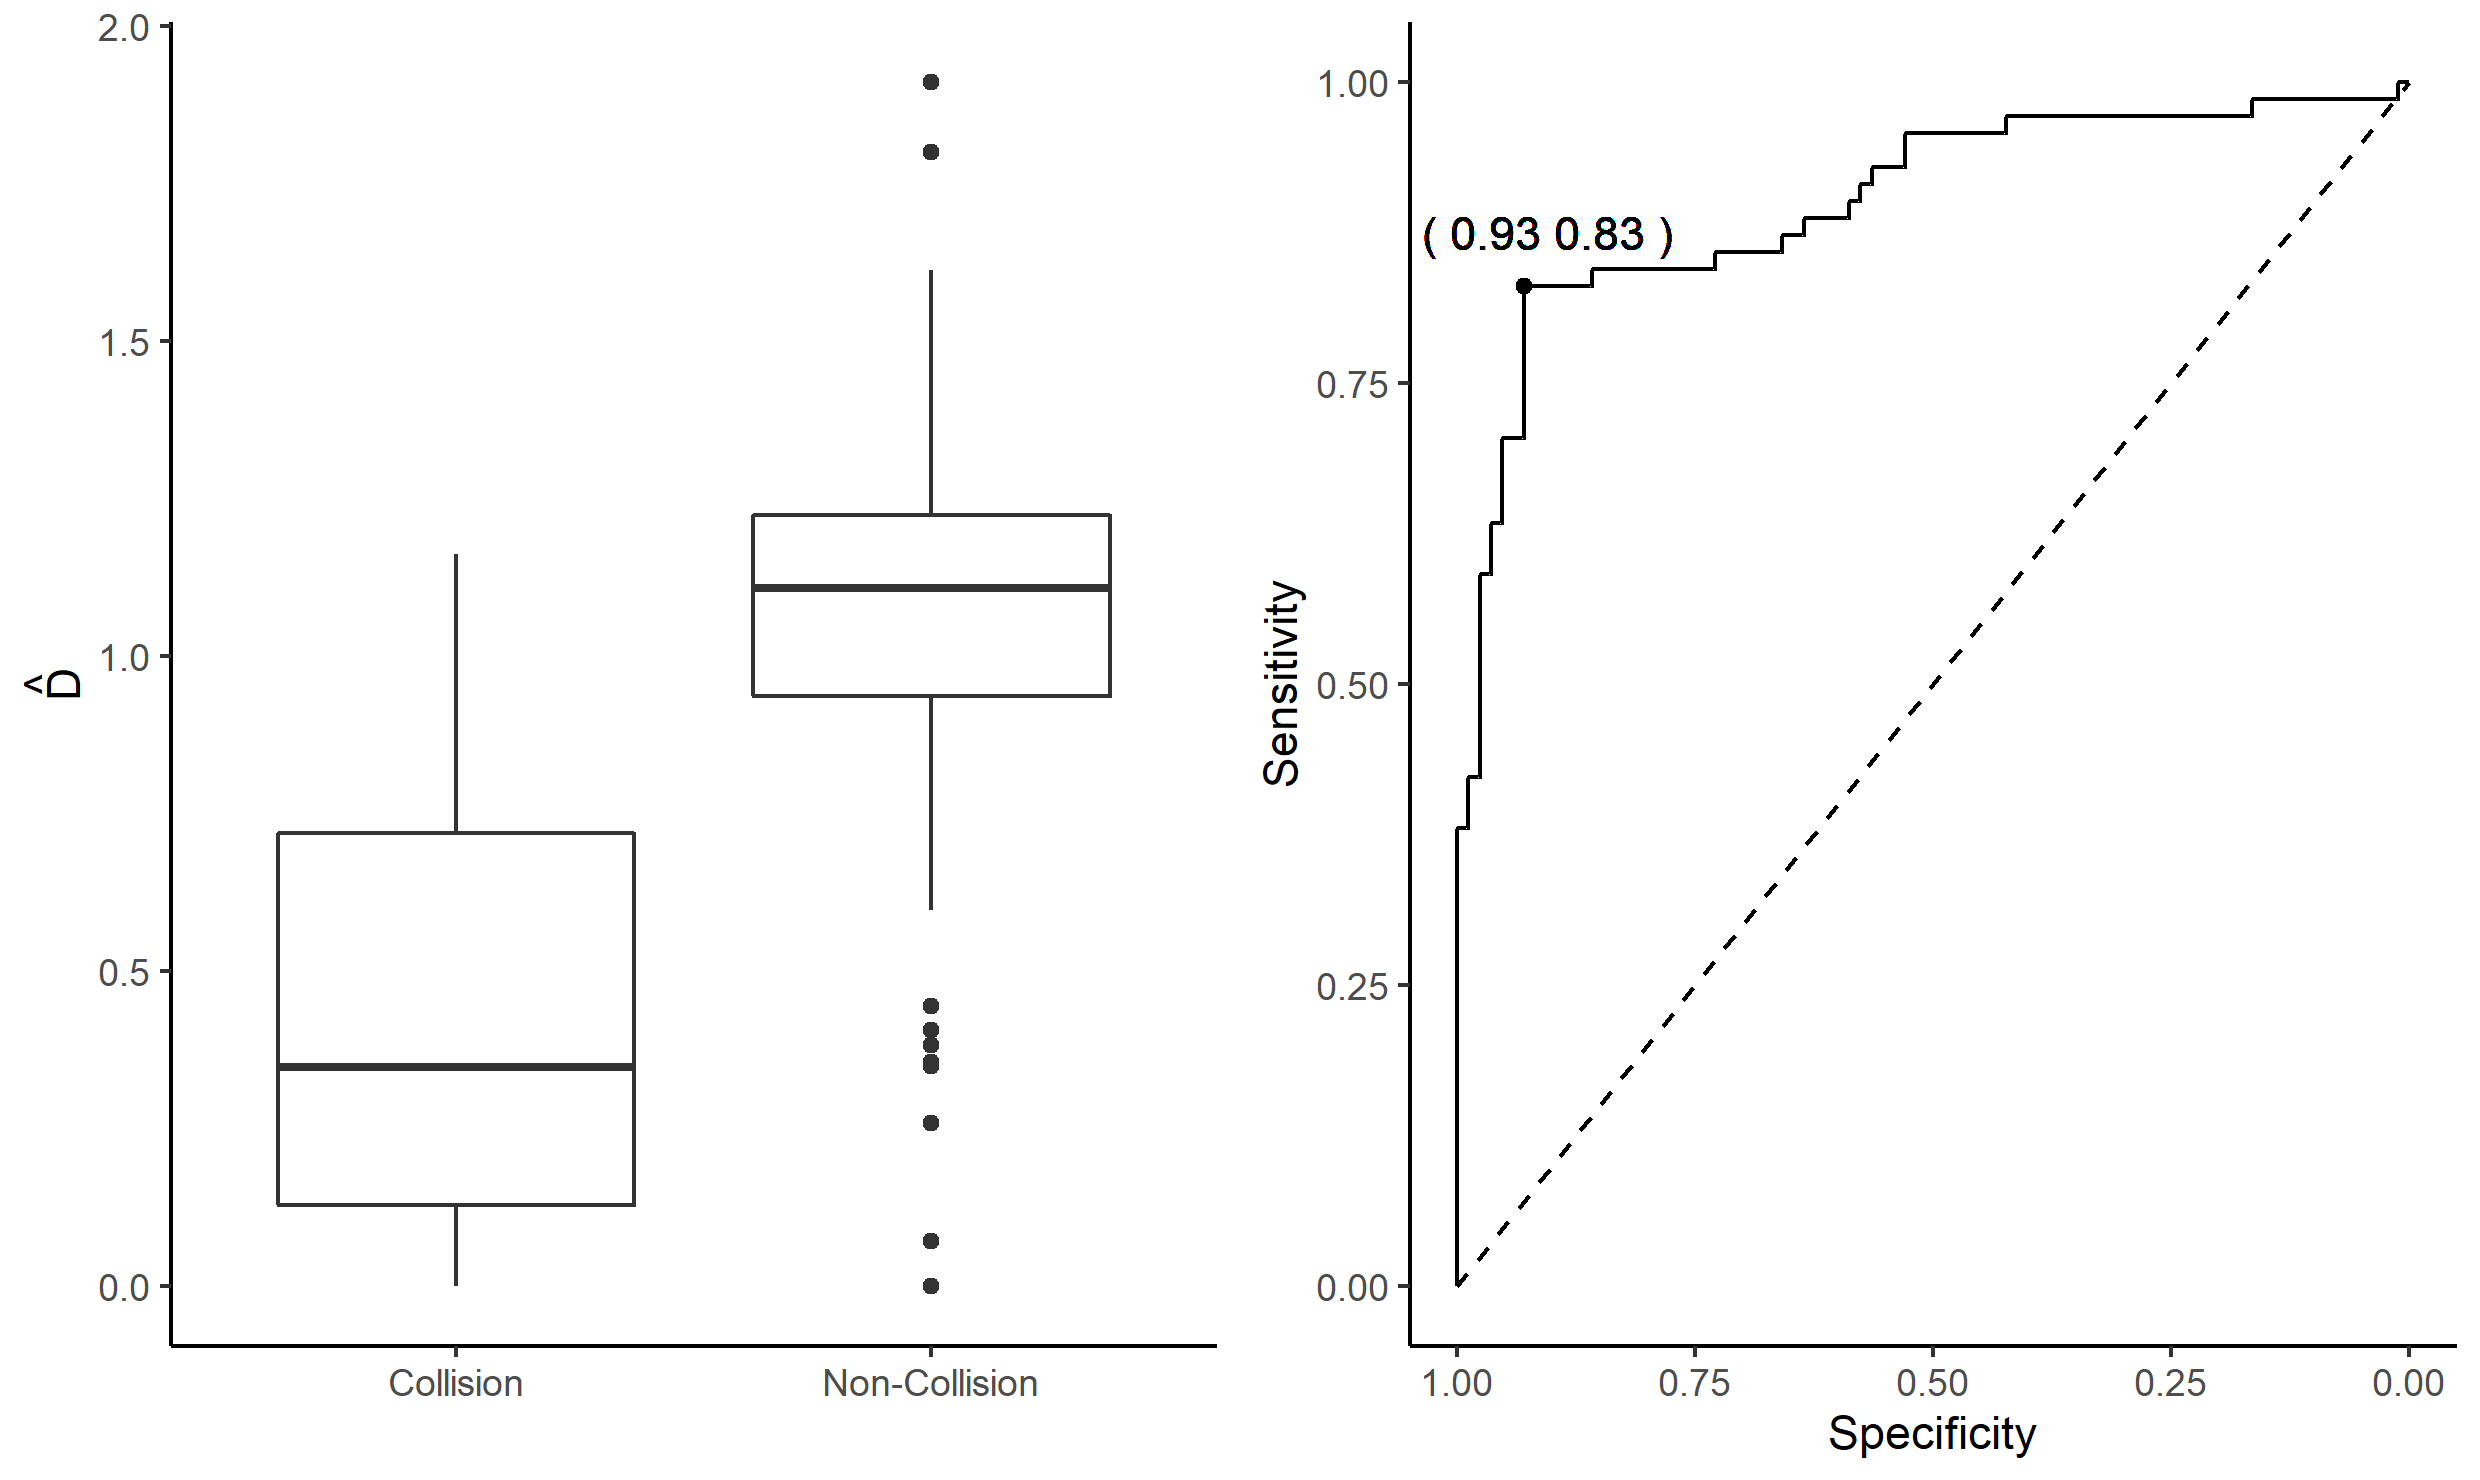
\includegraphics[width=\textwidth]{fig2.png}
\caption{The left panel shows the distribution of $\hat{D}$ by collision, the right panel shows the ROC Curve of $\hat{D} $ as classifier of collision.  The sensitivity and specificity corresponding to a decision threshold of $\hat{D} = 0.9$ are highlighted on the ROC Curve.}
\label{figure 2}
\end{figure}

Figure~\ref{figure 2} displays a the distribution of $\hat{D}$ values for collsions and non-collisions, as well as the Receiver Operating Characteristic (ROC) curve illustrating the diagnostic ability of $\hat{D}$.  A decision boundary of $\hat{D} = 0.9$ yields 93$\%$ specificity and 83$\%$ sensitivity, implying that the measure will correctly identify 93$\%$ of collisions as such, while only misclassifying 17$\%$ of non-collisions as collisions.  Additionally the Area Under the Curve (AUC) of the ROC curve is 0.891, affirming $\hat{D}$ as a good classifier for a range of decision thresholds, and indicating expectional classification performance.

\subsection{Evaluating Alert Characteristics}

As previously indicated, the intent of this study was to determine in the impact of the haptic alert characteristics INT, IPI, and DIP on how the participant reacted to the incursion vehicle. Visual inspection shows that INT might have a relationship with whether a collision occured, a natural outcome of interest.  Additionally, INT also appears related to $\hat{D}$, an alternative measure for quantifying the participant's reaction.

\begin{figure}[h!]
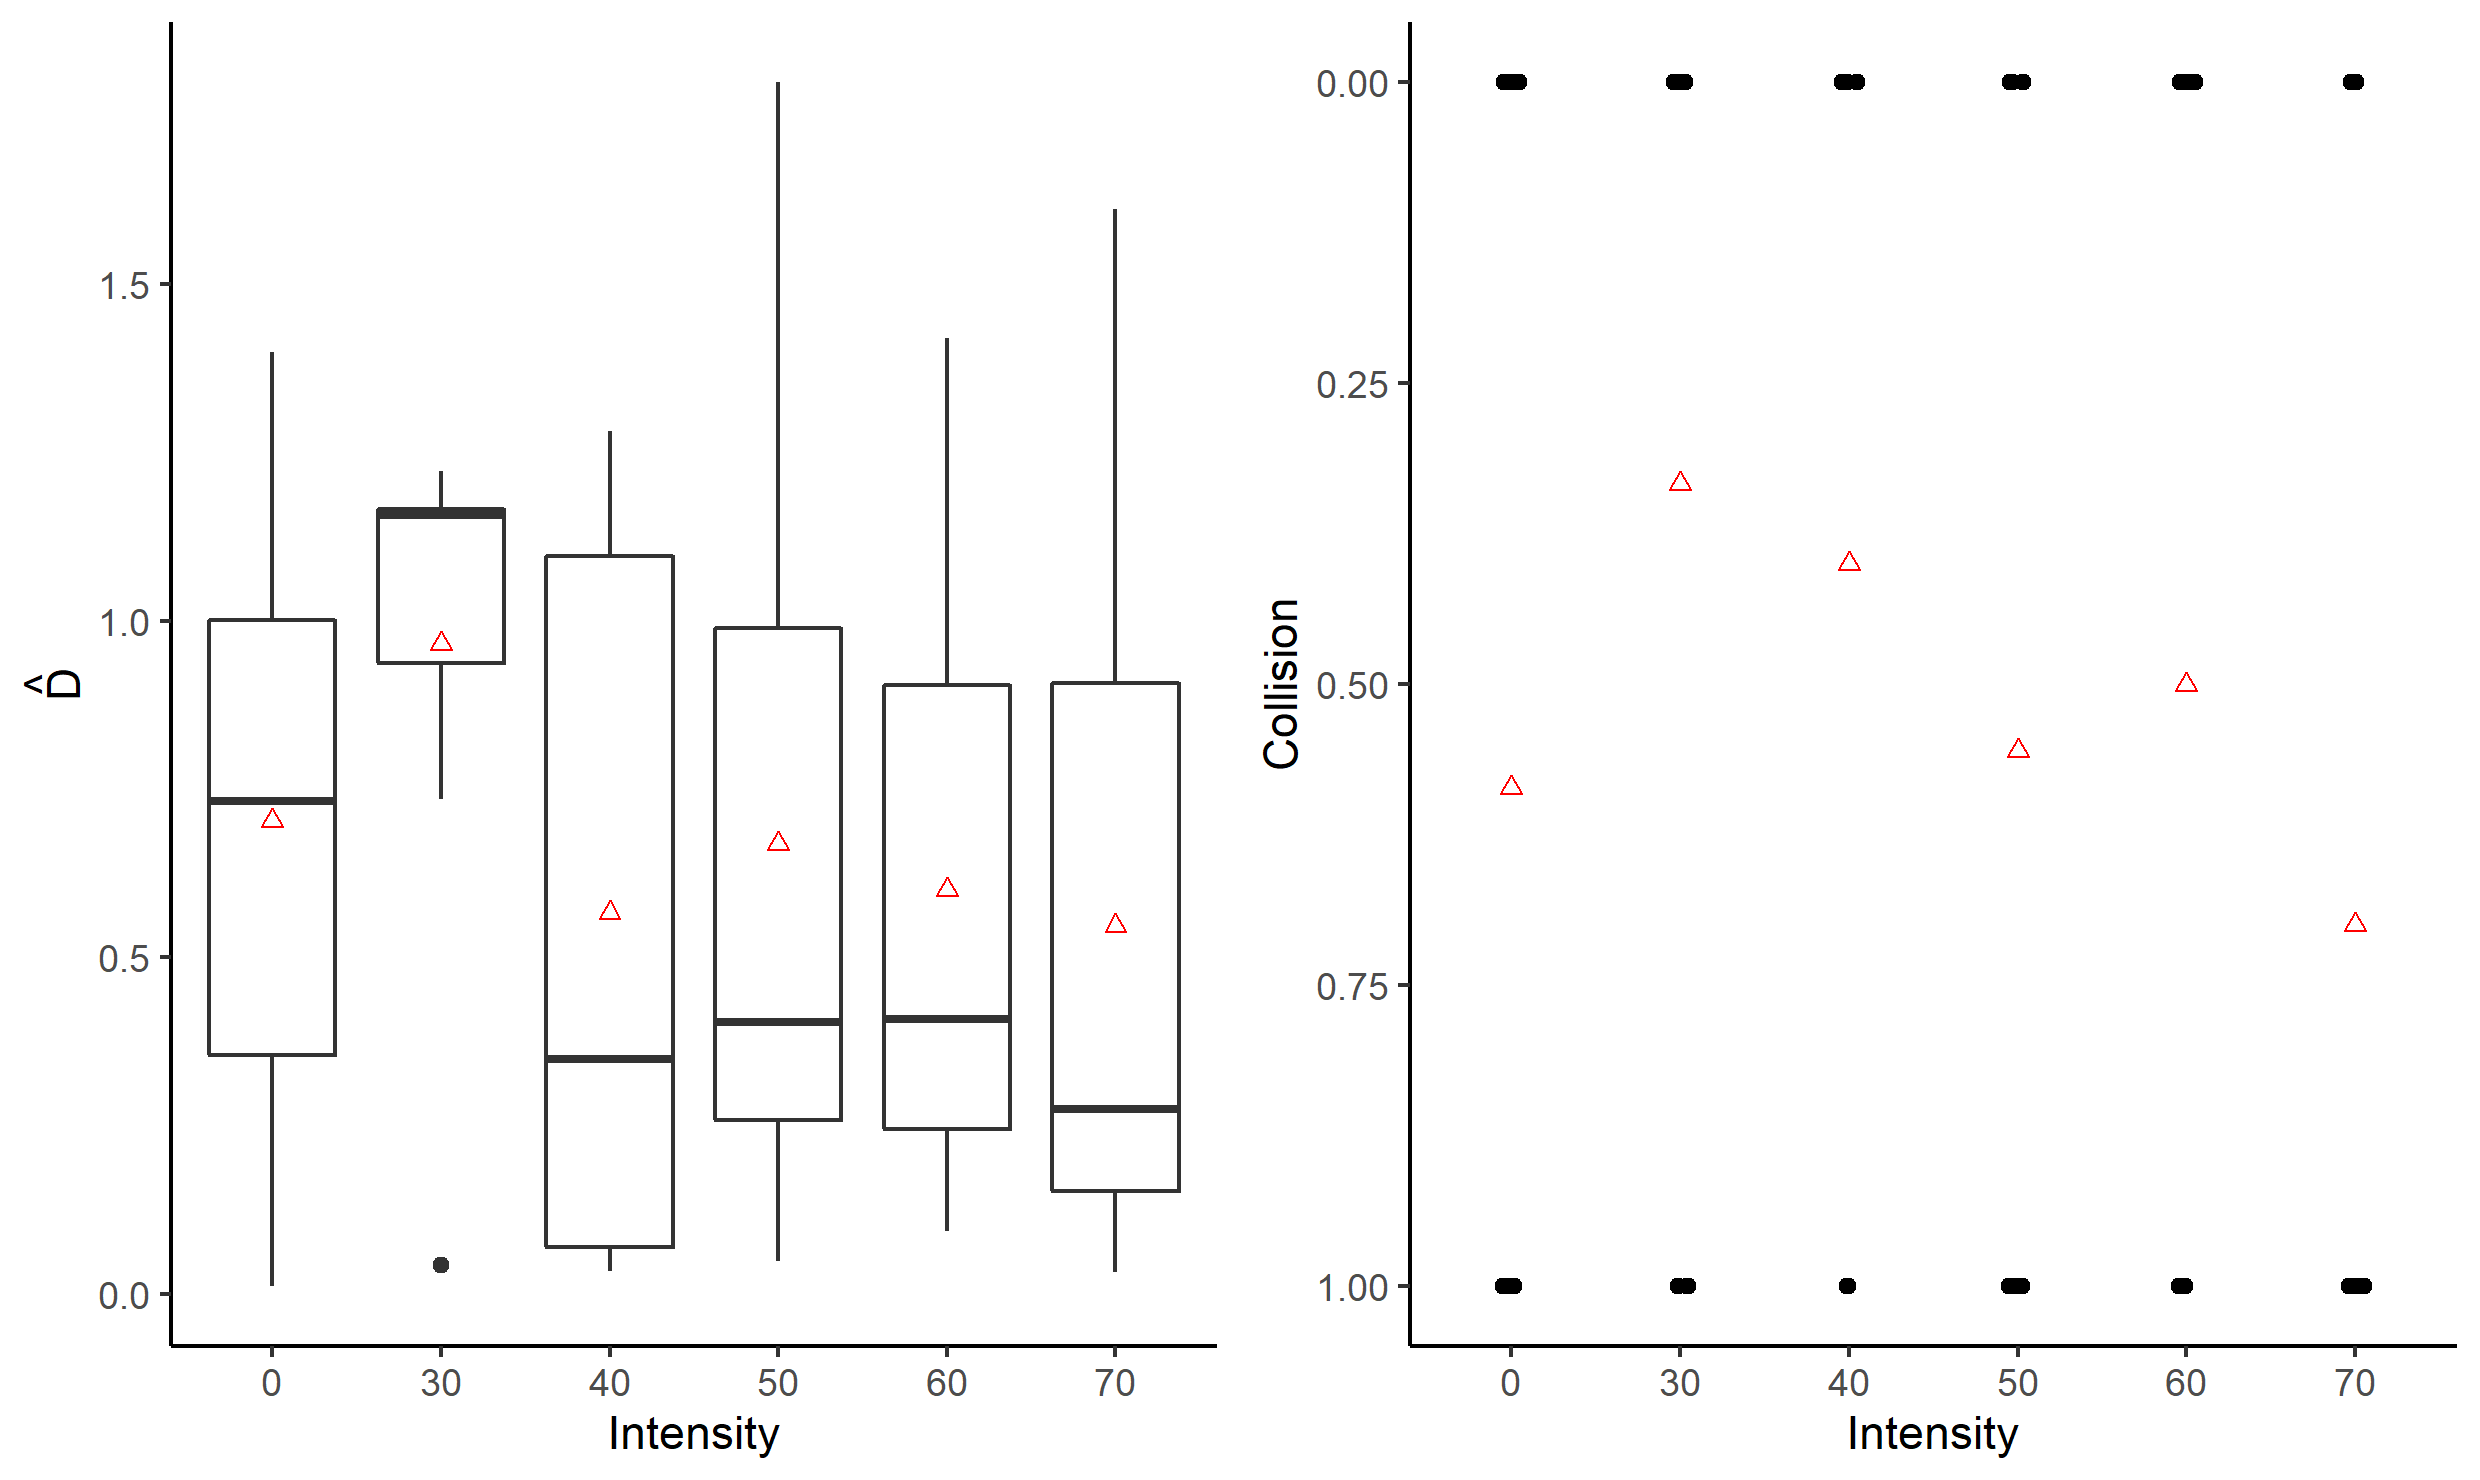
\includegraphics[width=\textwidth]{fig3.png}
\caption{Trends in Alert Intensity using $\hat{D}$ and Collision}
\label{figure 3}
\end{figure}

Figure~\ref{figure 3} illustrates differences in response for different levels of intensity, with IPI and DIP set at their default values.  The expection is INT $=0$, which represents the control group where no alert occurred.  These graphs suggest that lower INT levels tended to result in fewer collisions, relative to both the control group and the higher INT conditions.

We might more formally assess the impact of these chracteristics using statistical modeling.  Here we use logistic regression to model whether a collision occurred using the alert characteristics as explanatory variables.  For comparison, we use linear regression to model the $\hat{D}$ using the alert characteristics.

\begin{table}[hbt]
\centering
\begin{tabular}{rlllrlr}
  \hline
 & Outcome & Family & Link & $\chi^2$ & df & $p$-value \\ 
  \hline
 & $\hat{D} $ & Gaussian & Identity & 3.29 & 1 & 0.07 \\ 
  & Collision & Binomial & Logit & 2.42 & 1 & 0.12 \\ 
   \hline
\end{tabular}
\caption{Likelihood ratio test results for INT}
\label{table 1}
\end{table}


Table~\ref{table 1} shows the likelihood ratio tests for INT in the respective linear and logistic regression models with INT, IPI and DIP as predictors, and $\hat{D}$ or collision as the response variable. Both show some indication that INT is an important predictor, but the statistical confidence in the effect of INT differs. Although neither $p$-values reaches the convential significance threshold of $\alpha = 0.05$, the $p$-value when using $\hat{D}$ as an outcome is nearly halved.  Thus, the added information contained $SDCA$ considerably improves the statistical power in this application.

\section{Discussion}

TCA is the time to closest approach of two vehicles with set reaction profiles and a fixed reference point. In the event of a collision, TCA is an effective method of determining the time at which a collision occurs relative to the start of the reaction. Therefore, in case of collisions, smaller values of TCA indicate greater imminence of the collision. However, we have three salient criticisms of the metric:
\begin{enumerate}
    \item Comparing across different crash data poses challenges as the reference point across all data needs to be fixed in order to get a meaningful interpretation of TCA for the data. This is a substantial limitation, as reference points are not generally consistent across real-world crash situations.
    \item TCA has limited applicability in the absence of a collision across multiple scenarios, as it is not reflective of imminence of danger. For example, a TCA of 4s does not distinguish between two sets of vehicles that are 5m and 15m apart from each other at TCA. Therefore, TCA does not uniformly reflect proximity to collision.
    \item In case of a collision, TCA does not include information about severity of a collision and hence, does not distinguish between major and minor collisions.
\end{enumerate}
SDCA addresses these limitations. SDCA, or standardized degree of collision avoidance can be understood as the proximity to collision of two vehicles. SDCA turns the binary variable collision into a spectrum of positive values. By design, values farther away from 0 indicate greater levels of safety from collision.\\ SDCA is capable of quantitatively measuring the degree of collision (or non-collision) between two vehicles with set reaction profiles. This solves for our second and third criticisms of TCA. SDCA naturally equalizes different reference points because it uses delay in reaction times, rather than the time from the reference point itself. For example, if two vehicles are on track to collide and are currently two seconds away from their collision point their TCA is 2s while SDCA is 0. If we change the reference point to when the two vehicles are only 1s away from each other, their TCA becomes 1 while the SDCA remains 0. This simple example illustrates how SDCA is not reference-point dependent, which allows different scenario to have their own reference points while still providing for meaningful comparisons across scenarios.\\
In Sec (ref-methods) we present two separate SDCA calculations, one treating vehicles as points and another treating them as rectangles. We argue that both have utility.\\
The first method is point based calculation of SDCA. We conduct our analysis using this method, Each point used is located in the center of one of the two vehicles. $\hat{D} = 0$ in this interpretation would indicate a collision of the centers of the vehicles, the most severe collision scenario theoretically possible. Since SDCA comprises of a spectrum of positive values, increasing values indicate decreasing severity of collision, and after a point, decreasing proximity to collision. In applying the metric to data, we set data-dependent thresholds to interpret the extent of collisions and non-collisions for different participants. As illustrated in figure \ref{figure 4}, the values in SDCA can be interpreted according to their position in the spectrum.
\begin{figure}[h!]
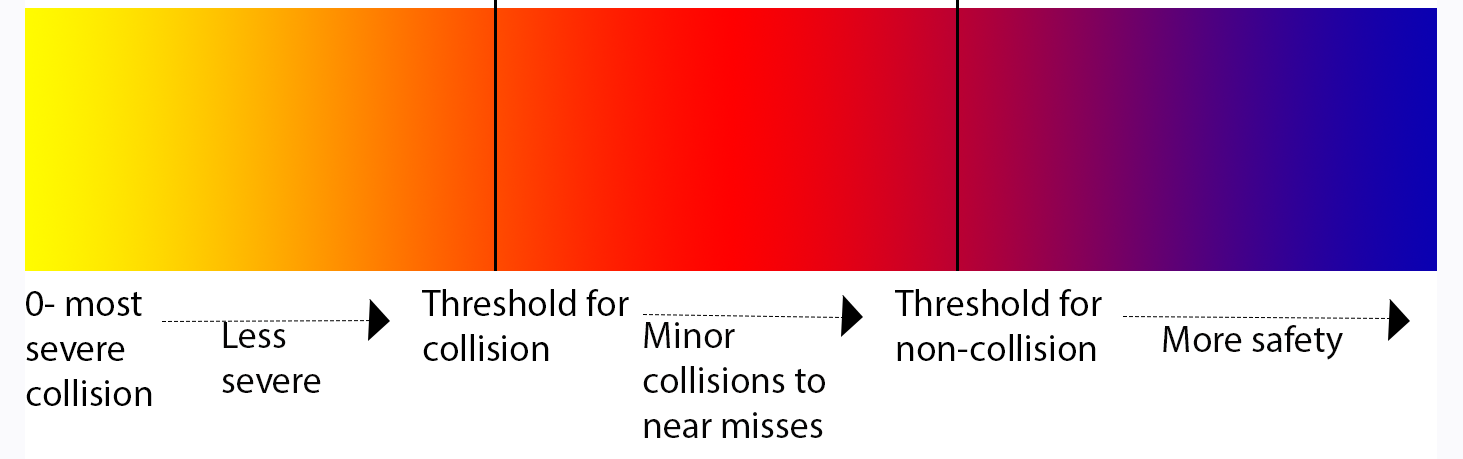
\includegraphics[width = 12cm, height = 3 cm]{discussion_1.png}
\label{figure 4}
\end{figure}\\
As figure 1 indicates, the boxplots of $\hat{D}$ for collision and non-collision differ greatly. We use their mean values as thresholds to interpret different SCDA values obtained.
Object based calculation- All non-zero values of SCDA signify non-collision, with increasing values indicating less proximity to collision. If SCDA is 0, we can identify the point-edge pair that collides by observing the distance function that first returns 0. However, this information is not encoded in SCDA itself but in its calculation.
Both versions of SCDA have their strengths. Point based calculation of SCDA gives a range of values that determine severity and proximity of collision, which makes it a superior method for data analysis. Conversely, object based calculation of SCDA has potential of revealing the position of crash. Also, since the object based calculation sets a clear threshold of non-collisions (all non-zero values), it might do a better job at forecasting collisions than point based calculations of SCDA.\\
This metric is good at forecasting the extent of collision and non-collision that a set of vehicles encounter, as illustrated in section 3. There are multiple ways to use SDCA for forecasting.\\
One method follows the calculation illustrated in section 3.2. The method requires estimation of reaction profiles at a fixed start point for a set of vehicles and use of the estimated profile to calculate SDCA. In real world scenarios for forecasting collision from a fixed start point, there is a lag in our metric to get accurate estimates. This lag is still shorter than the length of reaction, and some forecasting power is sacrificed, but not lost. The advantage of using this method is that, as only a single SDCA value is obtained for a set of vehicles, the estimated SDCA is relatively simple to calculate and interpret for a scenario. Hence, it allows for comparisons across different V2V collision scenarios, as depicted in section 3.3. SDCA estimated through this method is also a good approximation of the true SDCA if the vehicles' reactions do not alter significantly.\\
Another method for calculation of SDCA is to treat every instance of time after the imminence of the threat of collision as a separate reference point and determine the vehicles' reaction profiles instantaneously. This makes SDCA a dynamic measure that forecasts the occurrence of collision based on a vehicle's immediate reaction profile. This method is optimal for real-world collision avoidance as it reflects the threat of collision posed to a vehicle at every instance. Hence, a driver can modify their reaction profile repeatedly to obtain larger SDCA values and avoid a collision. However, because this method gives a series of SDCA values for every time frame, its interpretability for a scenario is limited. This hinders comparisons across multiple V2V scenarios as well.\\
As mentioned above, using object based calculation of SDCA might be better at forecasting as it considers all points of collision between two vehicles. By having a clear threshold that separates collisions and non-collisions, it can more accurately help vehicles avoid collisions entirely. Conversely, if a collision is imminent, point based calculation of SDCA would be useful as it consists of a spectrum of values that separate severe collisions from mild collisions. In a real-world situation, therefore, both calculations of SDCA should be used in tandem.\\
As demonstrated in section 3.4, SDCA improves statistical analysis, as compared to a dummy variable for collision. By using a continuous variable, we are able to distinguish between collisions of different levels of severity and therefore get a stronger analysis. For example, a head-on collision and a mild scrape would both be classified as a collision, when their levels of severity differ greatly. This distinction is visible using SDCA, making it a more robust response variable. Figure 3 and table 1 highlight the superiority of SDCA to a binary collision variable, which depict similar trends for INT across both response variables, but produce more statistically significant results with SDCA as the response. Using the point wise calculation of SDCA is better for analysis because it incorporates that distinction for both, collisions and non-collisions.
\section{Conclusion}
We create time-based metric that measures proximity to collisions in real-world, we adapt time to closest approach (TCA) by Schwarz to create the standardized degree of collision avoidance (SDCA). SDCA is a measure of proximity of collision, and converts the binary variable collision into a range of values. We use point wise and object wise calculations to determine SDCA. Both methods have different applications. SDCA can be used to forecast the occurrence or non-occurrence of collision as well as replace the binary collision variable to strengthen analysis.

\bibliography{references} 

\end{document} 

